% Graphics for slide 4, in the order the PDF draws them.
\begin{tikzpicture}[remember picture, overlay, x=1bp, y=-1bp,
  shift={(current page.north west)}]
\path[fill=cFFFFFF] (0,0) rectangle (960,540);
\path[fill=cF2F2F2,even odd rule] (56.69,116.33) ..controls(56.69,112.3)and(59.96,109.03)..(64,109.03) --(301.46,109.03) ..controls(305.49,109.03)and(308.76,112.3)..(308.76,116.33) --(308.76,245.73) ..controls(308.76,249.76)and(305.49,253.03)..(301.46,253.03) --(64,253.03) ..controls(59.96,253.03)and(56.69,249.76)..(56.69,245.73) --(56.69,116.33);
\node[anchor=north west, inner sep=0pt] at (56.69,109.03) {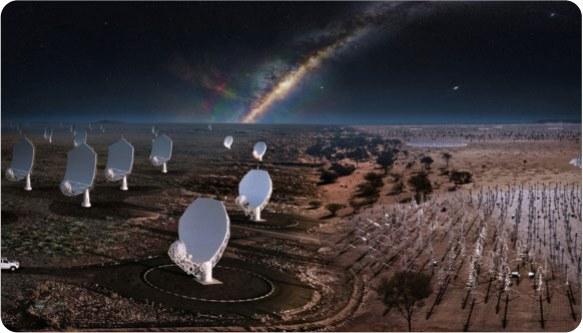
\includegraphics[width=252.43bp, height=144bp]{figures/fundamentals-of-hpc/p04-1.jpg}};
\node[anchor=north west, inner sep=0pt] at (56.69,477.21) {
\includegraphics[width=73.42bp, height=37.42bp]{figures/fundamentals-of-hpc/p03-1.png}};
\path[fill=cEE7628,even odd rule] (91.83,235.85) --(205.44,235.85) ..controls(212.42,235.85)and(218.08,239.39)..(218.08,243.76) --(218.08,265.92) ..controls(218.08,270.29)and(212.42,273.84)..(205.44,273.84) --(91.83,273.84) ..controls(84.85,273.84)and(79.19,270.29)..(79.19,265.92) --(79.19,243.76) ..controls(79.19,239.39)and(84.85,235.85)..(91.83,235.85);
\path[fill=cEE7628,even odd rule] (57.18,55.73) ..controls(57.96,55.73)and(58.6,56.37)..(58.6,57.15) --(58.6,85.5) ..controls(58.6,86.28)and(57.96,86.91)..(57.18,86.91) ..controls(56.4,86.91)and(55.76,86.28)..(55.76,85.5) --(55.76,57.15) ..controls(55.76,56.37)and(56.4,55.73)..(57.18,55.73);
\path[fill=cF2F2F2,even odd rule] (56.69,291.83) ..controls(56.69,287.8)and(59.96,284.53)..(64,284.53) --(301.46,284.53) ..controls(305.49,284.53)and(308.76,287.8)..(308.76,291.83) --(308.76,421.22) ..controls(308.76,425.26)and(305.49,428.53)..(301.46,428.53) --(64,428.53) ..controls(59.96,428.53)and(56.69,425.26)..(56.69,421.22) --(56.69,291.83);
\node[anchor=north west, inner sep=0pt] at (56.69,284.53) {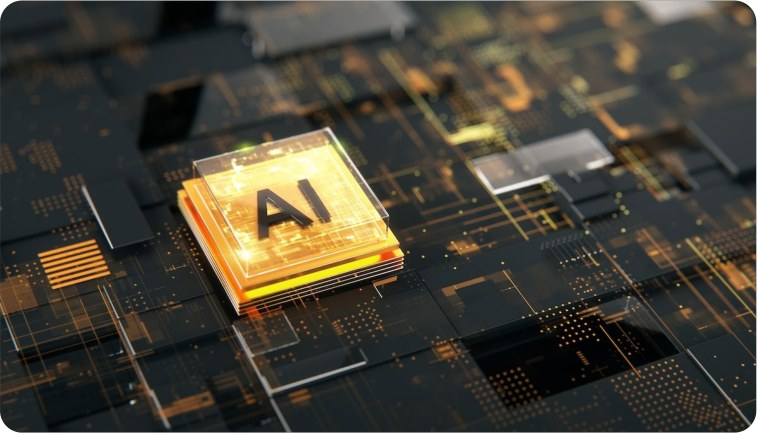
\includegraphics[width=252.07bp, height=144.1bp]{figures/fundamentals-of-hpc/p04-3.jpg}};
\path[fill=cF6DA44,even odd rule] (91.83,411.92) --(205.44,411.92) ..controls(212.42,411.92)and(218.08,415.41)..(218.08,419.72) --(218.08,441.54) ..controls(218.08,445.85)and(212.42,449.34)..(205.44,449.34) --(91.83,449.34) ..controls(84.85,449.34)and(79.19,445.85)..(79.19,441.54) --(79.19,419.72) ..controls(79.19,415.41)and(84.85,411.92)..(91.83,411.92);
\path[fill=cF2F2F2,even odd rule] (353.96,116.33) ..controls(353.96,112.3)and(357.23,109.03)..(361.27,109.03) --(598.73,109.03) ..controls(602.77,109.03)and(606.04,112.3)..(606.04,116.33) --(606.04,245.73) ..controls(606.04,249.76)and(602.77,253.03)..(598.73,253.03) --(361.27,253.03) ..controls(357.23,253.03)and(353.96,249.76)..(353.96,245.73) --(353.96,116.33);
\node[anchor=north west, inner sep=0pt] at (353.96,109.03) {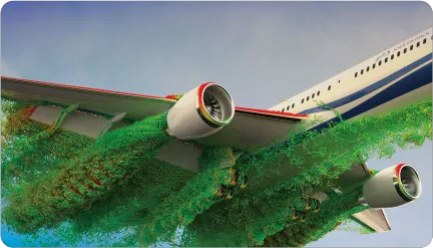
\includegraphics[width=252.07bp, height=144.12bp]{figures/fundamentals-of-hpc/p04-4.jpg}};
\path[fill=c2CA055,even odd rule] (389.1,235.85) --(502.71,235.85) ..controls(509.69,235.85)and(515.35,239.39)..(515.35,243.76) --(515.35,265.92) ..controls(515.35,270.29)and(509.69,273.84)..(502.71,273.84) --(389.1,273.84) ..controls(382.12,273.84)and(376.46,270.29)..(376.46,265.92) --(376.46,243.76) ..controls(376.46,239.39)and(382.12,235.85)..(389.1,235.85);
\path[fill=cF2F2F2,even odd rule] (353.96,291.83) ..controls(353.96,287.8)and(357.23,284.53)..(361.27,284.53) --(598.73,284.53) ..controls(602.77,284.53)and(606.04,287.8)..(606.04,291.83) --(606.04,421.22) ..controls(606.04,425.26)and(602.77,428.53)..(598.73,428.53) --(361.27,428.53) ..controls(357.23,428.53)and(353.96,425.26)..(353.96,421.22) --(353.96,291.83);
\node[anchor=north west, inner sep=0pt] at (353.96,284.53) {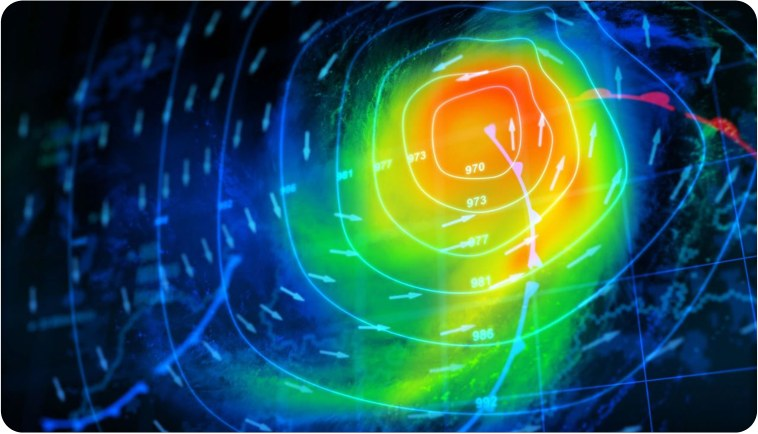
\includegraphics[width=252.07bp, height=144.15bp]{figures/fundamentals-of-hpc/p04-5.jpg}};
\path[fill=c7B2882,even odd rule] (389.1,411.92) --(502.71,411.92) ..controls(509.69,411.92)and(515.35,415.41)..(515.35,419.72) --(515.35,441.54) ..controls(515.35,445.85)and(509.69,449.34)..(502.71,449.34) --(389.1,449.34) ..controls(382.12,449.34)and(376.46,445.85)..(376.46,441.54) --(376.46,419.72) ..controls(376.46,415.41)and(382.12,411.92)..(389.1,411.92);
\path[fill=cF2F2F2,even odd rule] (651.24,116.33) ..controls(651.24,112.3)and(654.51,109.03)..(658.54,109.03) --(896,109.03) ..controls(900.04,109.03)and(903.31,112.3)..(903.31,116.33) --(903.31,245.73) ..controls(903.31,249.76)and(900.04,253.03)..(896,253.03) --(658.54,253.03) ..controls(654.51,253.03)and(651.24,249.76)..(651.24,245.73) --(651.24,116.33);
\node[anchor=north west, inner sep=0pt] at (651.24,109.03) {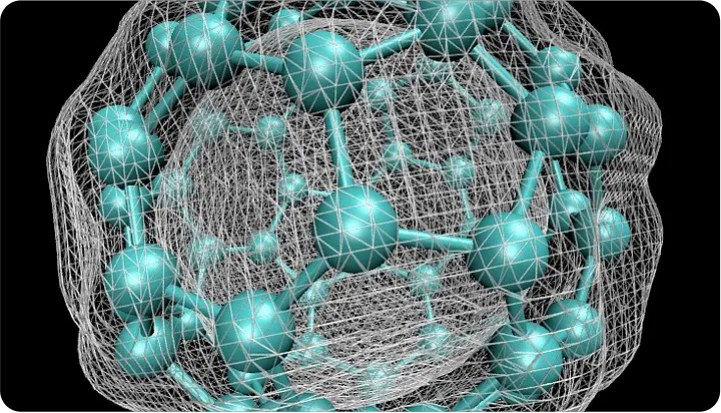
\includegraphics[width=252.07bp, height=144.24bp]{figures/fundamentals-of-hpc/p04-6.jpg}};
\path[fill=c177ABF,even odd rule] (686.37,235.85) --(799.99,235.85) ..controls(806.96,235.85)and(812.62,239.39)..(812.62,243.76) --(812.62,265.92) ..controls(812.62,270.29)and(806.96,273.84)..(799.99,273.84) --(686.37,273.84) ..controls(679.39,273.84)and(673.74,270.29)..(673.74,265.92) --(673.74,243.76) ..controls(673.74,239.39)and(679.39,235.85)..(686.37,235.85);
\path[fill=cF2F2F2,even odd rule] (651.24,291.83) ..controls(651.24,287.8)and(654.51,284.53)..(658.54,284.53) --(896,284.53) ..controls(900.04,284.53)and(903.31,287.8)..(903.31,291.83) --(903.31,421.22) ..controls(903.31,425.26)and(900.04,428.53)..(896,428.53) --(658.54,428.53) ..controls(654.51,428.53)and(651.24,425.26)..(651.24,421.22) --(651.24,291.83);
\node[anchor=north west, inner sep=0pt] at (651.24,284.53) {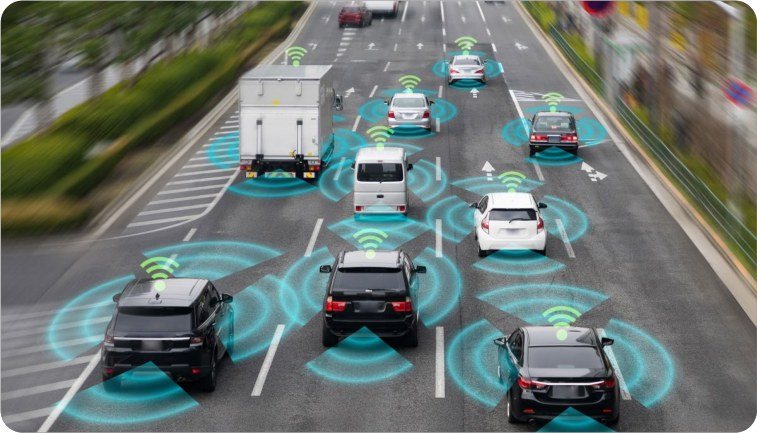
\includegraphics[width=252.07bp, height=144.1bp]{figures/fundamentals-of-hpc/p04-7.jpg}};
\path[fill=cE7303A,even odd rule] (686.37,411.92) --(799.99,411.92) ..controls(806.96,411.92)and(812.62,415.41)..(812.62,419.72) --(812.62,441.54) ..controls(812.62,445.85)and(806.96,449.34)..(799.99,449.34) --(686.37,449.34) ..controls(679.39,449.34)and(673.74,445.85)..(673.74,441.54) --(673.74,419.72) ..controls(673.74,415.41)and(679.39,411.92)..(686.37,411.92);
\end{tikzpicture}
